\documentclass[sigconf,authordraft]{acmart}

%%
%% \BibTeX command to typeset BibTeX logo in the docs
\AtBeginDocument{%
  \providecommand\BibTeX{{%
    \normalfont B\kern-0.5em{\scshape i\kern-0.25em b}\kern-0.8em\TeX}}}

%% Rights management information.  This information is sent to you
%% when you complete the rights form.  These commands have SAMPLE
%% values in them; it is your responsibility as an author to replace
%% the commands and values with those provided to you when you
%% complete the rights form.
\setcopyright{acmcopyright}
\copyrightyear{2020}
\acmYear{2020}
%\acmDOI{10.1145/1122445.1122456}

%% These commands are for a PROCEEDINGS abstract or paper.
\acmConference[PEARC '20]{PEARC '20}{July 26-30, 2020}{Portland, OR }
%\acmBooktitle{Woodstock '18: ACM Symposium on Neural Gaze Detection,
%  June 03--05, 2018, Woodstock, NY}
%\acmPrice{15.00}
%\acmISBN{978-1-4503-XXXX-X/18/06}


%%
%% Submission ID.
%% Use this when submitting an article to a sponsored event. You'll
%% receive a unique submission ID from the organizers
%% of the event, and this ID should be used as the parameter to this command.
%%\acmSubmissionID{123-A56-BU3}

%%
%% The majority of ACM publications use numbered citations and
%% references.  The command \citestyle{authoryear} switches to the
%% "author year" style.
%%
%% If you are preparing content for an event
%% sponsored by ACM SIGGRAPH, you must use the "author year" style of
%% citations and references.
%% Uncommenting
%% the next command will enable that style.
%%\citestyle{acmauthoryear}

%%
%% end of the preamble, start of the body of the document source.
\begin{document}

%%
%% The "title" command has an optional parameter,
%% allowing the author to define a "short title" to be used in page headers.
\title{Benchmark informed software upgrades at Quest-NUiT}

%%
%% The "author" command and its associated commands are used to define
%% the authors and their affiliations.
%% Of note is the shared affiliation of the first two authors, and the
%% "authornote" and "authornotemark" commands
%% used to denote shared contribution to the research.
\author{Sajid Ali}
\orcid{0000-0003-2186-4636}
\affiliation{%
  \institution{Applied Physics, Northwestern University}
  \streetaddress{2145 Sheridan Road}
  \city{Evanston}
  \state{Illinois}
  \postcode{60208}
}
\email{sajidsyed2021@u.northwestern.edu}

\author{Alper Kinaci}
\affiliation{%
\institution{NUiT RCS, Northwestern University}
  \streetaddress{2145 Sheridan Road}
  \city{Evanston}
  \state{Illinois}
  \postcode{60208}
  }
\email{akinaci@northwestern.edu}

%%
%% By default, the full list of authors will be used in the page
%% headers. Often, this list is too long, and will overlap
%% other information printed in the page headers. This command allows
%% the author to define a more concise list
%% of authors' names for this purpose.
%%\renewcommand{\shortauthors}{Trovato and Tobin, et al.}

%%
%% The abstract is a short summary of the work to be presented in the
%% article.
\begin{abstract}
  We present the work performed at Quest, a high performance computing cluster at Northwestern University regarding benchmarking of software perfromed to guide software upgrades. We performed extensive evaluation of all mpi libraries present on the system for functionality and performance in addition to testing a strategy to deploy architecture optimized software that can be loaded dynamically at runtime.
\end{abstract}

%%
%% The code below is generated by the tool at http://dl.acm.org/ccs.cfm.
%% Please copy and paste the code instead of the example below.
%%
\begin{CCSXML}
	<ccs2012>
	<concept>
	<concept_id>10011007.10011006.10011071</concept_id>
	<concept_desc>Software and its engineering~Software configuration management and version control systems</concept_desc>
	<concept_significance>500</concept_significance>
	</concept>
	<concept>
	<concept_id>10011007.10011006.10011073</concept_id>
	<concept_desc>Software and its engineering~Software maintenance tools</concept_desc>
	<concept_significance>300</concept_significance>
	</concept>
	</ccs2012>
\end{CCSXML}

\ccsdesc[500]{Software and its engineering~Software configuration management and version control systems}
\ccsdesc[300]{Software and its engineering~Software maintenance tools}

%%
%% Keywords. The author(s) should pick words that accurately describe
%% the work being presented. Separate the keywords with commas.
\keywords{software management, 	software builds, software automation}

%%
%% This command processes the author and affiliation and title
%% information and builds the first part of the formatted document.
\maketitle

\section{Introduction}

Quest is a heterogenous HPC cluster\cite{quest} at Northwestern University consisting of Intel Haswell/Broadwell/Skylake nodes with varying interconects which uses the slurm\cite{slurm} as resource manager and job scheduler (should we mention fairhsare ?). The cluster operates with very high uptimes and only shuts down once every academic year for maintainence (for approximately two weeks). While this high uptime is great for research throughput, it compresses critical maintaince tasks into those two weeks and makes the operators prioritize in place uprgrades over major redesigns. While such an operations scheme works in the short run, managing a large set of software stacks that were installed at various points in time becomes challenging. The software stack was kept stable even through maintaince cycles that involved major and minor OS upgrades. 

This has led to a bloated software stack with inconstent naming schemes for modules and executables that is challenging to continuously benchmark for functionality and performance. Thus, we are motivated to develop a strategy to maintain our software stacks that will enable us to provide functional and performant software for our users while reducing the maintainence and support workload for the operators and software specialists. In addition to the above, we also face an immediate need to make mpi launchers compatible with srun as a slurm update is on the agenda for the next downtime.

In this article we present the results of our benchmarking studies that inform our plans for deprecating modules and prelimary tests on our beta cluster for a strategy to deploy optimized builds for each architecture that are dynamically loaded at runtime based upon the nodelist for the job.

\section{MPI libraries}
Over time multiple builds of libraries proving the message passing interface\cite{mpi_3_1} functionality were installed. Some of these are quite old (before major OS version upgrades) and the naming scheme is inconsistent. Since none of these were installed with slurm support, we had to write a bash script to run the tests. The results are presented in the figure-abc.

\begin{figure}[h]
	\centering
	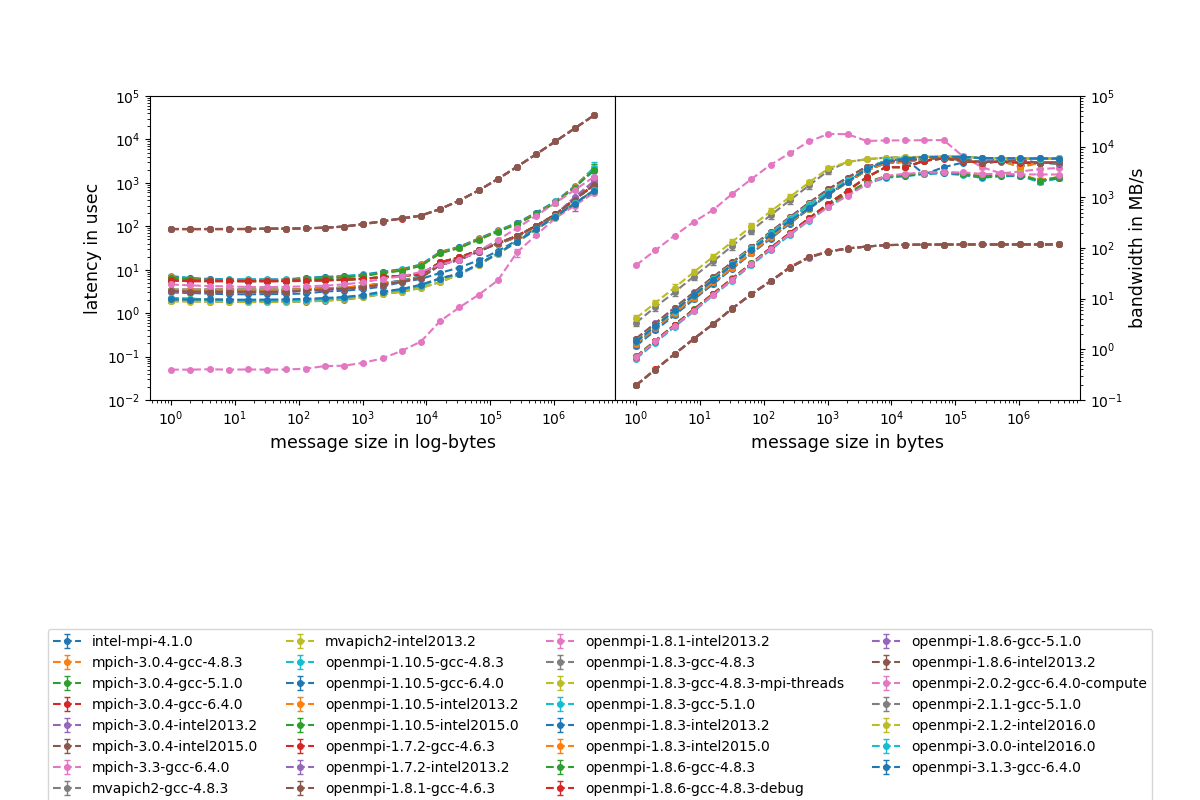
\includegraphics[width=\linewidth]{curr_mpi_combined}
	\caption{Benchmark of currently available mpi builds}
	\Description{Benchmark of currently available mpi builds}
\end{figure}

In total, $42\%$ of the available mpi libraries were faulty with $28\%$ being nonfunctional and the rest being nonperformant.

\begin{figure}[h]
	\centering
	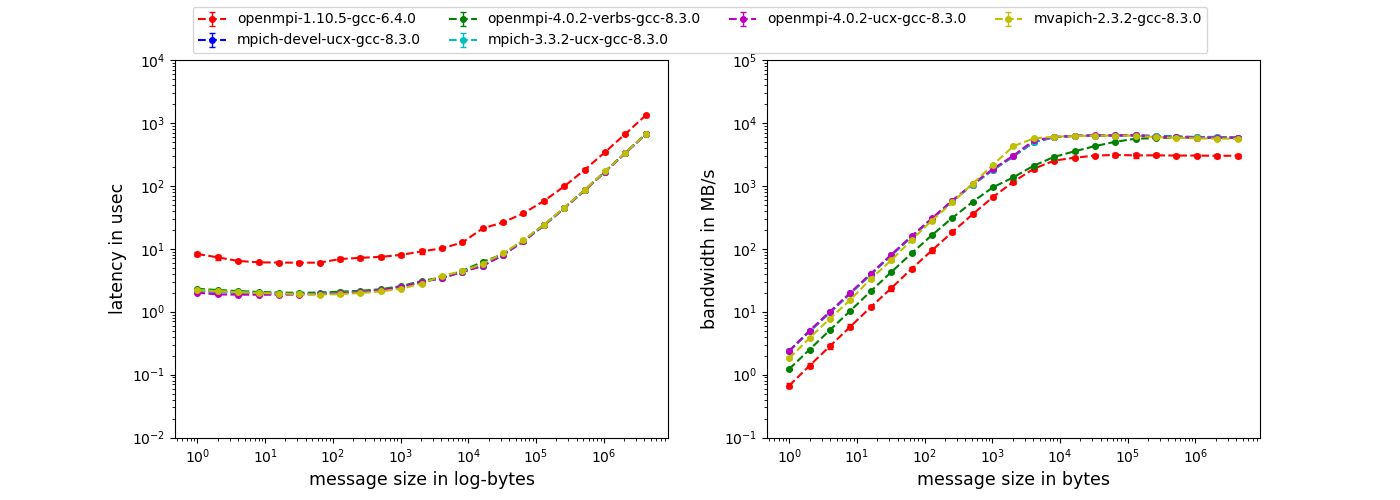
\includegraphics[width=\linewidth]{new_mpi}
	\caption{Benchmark of new mpi builds}
	\Description{Benchmark of new mpi builds}
\end{figure}


\subsection{Improvements}
 
Spack\cite{spack} was used to build new versions of mpi libraries with slurm support. This allows us to automate a large set of parameterized builds and eases the testing. Consistent with the literature we decided to use the "UCX" transport layer for all mpi libraries and to enable the "PMIx" plugin in slurm for better performance.

What is UCX ? How do we want to install it ?
What is PMIx ? How do we want to install it ?

\section{Node arch dependent software}

\subsection{benchmarks}
Table with benchmarks for LAMMPS/GROMACS.

\begin{table}
	\caption{Optimized builds on Haswell nodes}
	\label{tab:bench_apps}
	\begin{tabular}{ccl}
		\toprule
		Software &Current&Optimized\\
		\midrule
		LAMMPS & 765.8 timesteps/day&1013.4 timesteps/day\\
		GROMACS & 1.78 ns/day&2.00 ns/day\\
		\bottomrule
	\end{tabular}
\end{table}
 
Elaborate on the benchmark probelm, add citation.


\subsection{deployment strategy}
On Quest, users are not reuqired to choose a partition and the jobs are assigned to nodes dynamically based on availability. We plan to build each software package optimzed for all possible architectures and configure a task prolog script that sets the modulepath based on $SLURM\_NODELIST$ as shown below.

\begin{verbatim}
short_list=${SLURM_JOB_NODELIST##worker}
if [ $short_list == "01" ]
then
echo "export MODULEPATH=/home/path1"
fi
if [ $short_list == "02" ]
then
echo "export MODULEPATH=/home/path2"
fi
\end{verbatim}

This was tested on a virtual slurm cluster provisioned by four docker containers tied together via docker-compose. [cite].


\section{Conclusion}
Thus, an important study was conducted.

%%
%% The acknowledgments section is defined using the "acks" environment
%% (and NOT an unnumbered section). This ensures the proper
%% identification of the section in the article metadata, and the
%% consistent spelling of the heading.
\begin{acks}
To Alex from NUiT for help, to various mailing lists and forums including but not limited to mpich-discuss, slurm-info, spack-users.
\end{acks}

%%
%% The next two lines define the bibliography style to be used, and
%% the bibliography file.
\bibliographystyle{ACM-Reference-Format}
\bibliography{pearc20}

%%
%% If your work has an appendix, this is the place to put it.
%\appendix
%\section{Research Methods}
%\subsection{Part One}
%Lorem ipsum dolor sit amet, consectetur adipiscing elit. Morbi
%\subsection{Part Two}
%Etiam commodo feugiat nisl pulvinar pellentesque. Etiam auctor sodales
%\section{Online Resources}
%Nam id fermentum dui. Suspendisse sagittis tortor a nulla mollis, in

\end{document}
\endinput
%%
%% End of file `sample-authordraft.tex'.
